This chapter introduces some fundamental background concepts in robot path planning that are essential for understanding the methods adopted in the subsequent chapters.

We first discuss the differences in kinematics among different types of robots and the necessity of designing a suitable trajectory representation respecting these differences prior to formulating a path planning problem. We talk about continuous-time trajectory representation using Cubic Splines and Bernstein polynomials, which are leveraged extensively in both our GPU-based multi-robot optimizer and the bi-level manipulator optimizer. Next, we introduce how to pose a trajectory optimization problem and explore two broad types of optimization - Gradient-based and Sampling-based. We contrast the performance of these two paradigms for various applications and then explore collision avoidance constraints to the trajectory optimization problem. Under standard collision avoidance techniques, we discuss two approaches - distance-based Collision Avoidance, and Time-scaling. We also coin a few standard evaluation metrics for judging the quality of a trajectory planned by an optimizer.

Next, we discuss Multi-Robot Path Planning, starting with real-world multi-agent systems and the challenges involved in extending standard path planning approaches directly to them. We analyze a few existing multi-robot path planners and discuss their advantages and weaknesses. Finally, we provide a brief introduction to batch trajectory optimization and commercial off-the-shelf GPU-based mathematical libraries to prime the reader for the next chapter on our GPU-accelerated optimizer.

Next, we move on to the problem of joint-space or end-effector space path planning for robot manipulators and discuss state-of-the-art optimization methods used for manipulator planning. We offer a detailed explanation of methods such as CHOMP\cite{CHOMP}, TrajOpt\cite{TrajOpt}, STORM\cite{STORM} and Cross-Entropy Methods(CEM)\cite{iCEM}. These optimization techniques form the backdrop for the Via-Point Stochastic Trajectory Optimization(VPSTO)\cite{VPSTO} method, which forms a crucial component in our bi-level optimization framework for push actions in manipulators.

\section{Mobile Robot Kinematics}

\subsection{Holonomic Robots}\label{sec:holonomic_robots}

For a robot with $n$ controllable degrees of freedom, it is considered holonomic if it is capable of moving in any of those $n$ dimensions, i.e., the number of degrees of freedom is equal to the number of controllable degrees of freedom. Let us demonstrate this with the help of an example. Considering an omnidirectional robot fitted with special wheels so that it is capable of moving in any direction on a 2-D plane. The 2-D kinematics equation for the robot that started moving from the point $(x_0, y_0)$ can, therefore, be written as follows:

\begin{subequations}
\begin{align}
x = x_0+\dot{x}*\delta t\\
y = y_0+\dot{y}*\delta t
\end{align}
\end{subequations}

where $\dot{x}$ and $\dot{y}$ denote the velocities in the two axes and $\delta t$ indicates a time step.
A few examples of common holonomic robots include drones (holonomic in 3-D), omnidirectional robots, etc.

\subsection{Non-holonomic Robots}

Non-holonomic robot systems are characterized by constraint equations that limit the degrees of freedom. Thus the permissible degrees of freedom for nonholonomic robot systems are less than the controllable degrees of freedom. A typical example of a non-holonomic system in 2-D is a differential drive mobile robot that is incapable of slipping in the lateral direction. The non-holonomic constraint is written as below:
\begin{equation}
\dot{y} = \dot{x}\tan{\theta}
\end{equation}

The controls for a non-holonomic system are given by the linear velocity $v$ and the angular velocity $\omega$, giving rise to the following kinematics equations:

\begin{subequations}
\begin{align}
x = x_0 + v\delta t\cos{(\theta_0+\int\omega\delta t)}\\
y = y_0 + v\delta t\sin{(\theta_0+\int\omega\delta t)}\\
\end{align}
\end{subequations} 

\section{Trajectory Representation}\label{sec:trajectory_rep}

A trajectory parameterized by time defines a sequence or a function mapping successive timestamps to the motion space of a system. It indicates the robot's state at a certain point in time. There are two broad methods of representing a trajectory mathematically, as discussed below:

\subsection{Continuous-time representation}

Here, a trajectory is represented as a function $f: t\mapsto S$ where $S$ denotes the motion space of a robot. The function $f$ and its derivatives should satisfy the trajectory bounds, i.e. the start and end states of the robot, as well as intermediate waypoint states. It also determines the shape of the curve fitting the start and goal points and forms a very important design choice in most path-planning applications. Some of the commonly used functions used to represent holonomic and non-holonomic mobile robot trajectories include:

\subsubsection{Cubic Spline}

The function $f$ is considered to be a 3rd-order polynomial in $t$ with four weights, as depicted below:

\begin{equation}
f(t) = w_0 + w_1 t + w_2 t^2 + w_3 t^3
\label{eqn:cubic_spline}
\end{equation}

To solve for the weights, we would require a minimum of four equations, i.e. four deterministic states of the robot at predefined timestamps. To give an idea, we could know start and goal position and velocity values $f(t_0)$, $f(t_f)$, $\dot{f(t_0)}$ and $\dot{f(t_f)}$ for a trajectory between time $t_0$ and $t_f$ forming the boundary state vector $A$ and solve the following system of linear equations using the basis polynomial matrix $B$ to compute the weights $W = [w_0, w_1, w_2, w_3]$.

\begin{subequations}
 \begin{align}
    \begin{bmatrix}
        w_0 & w_1 & w_2 & w_3 
    \end{bmatrix} \begin{bmatrix}
        1 & 1 & 0 & 0 \\
        t_0 & t_f & 1 & 1 \\
        t_0^2 & t_f^2 & 2t_0 & 2t_f \\
        t_0^3 & t_f^3 & 3t_0^2 & 3t_f^2
    \end{bmatrix} = \begin{bmatrix}
        f(t_0) & f(t_f) & \dot{f(t_0)} & \dot{f(t_f)}
    \end{bmatrix}
    \\
or, \qquad WB = A \label{eqn:LP}
\end{align}   
\end{subequations}



The above system of linear equations becomes over-constrained as the number of constraints on the trajectory increases, necessitating an increase in the degree of the polynomial. Another approach to the over-constrained problem would be to sample goal points along the trajectory and plan piecewise trajectories leading up to the final destination state.

\subsubsection{Bernstein Polynomials}
The trajectory can be represented as a linear combination of Bernstein basis polynomials \cite{bernstein_gen} coming from the Bezier curve. The $i$-th Bernstein basis polynomial of order $n$ is a real-valued function valued on $t \in [0,1]$ as follows:
\begin{equation}
    \boldsymbol{B_{i,n}(t)} = {n \choose i}t^{i}(1-t)^{n-i}, \qquad i = 0,1,...n
\end{equation}

Fig. \ref{fig:Bernstein_curv} depicts Bernstein basis polynomials of order-4. 

\begin{figure*}[t!]
    \centering
    \begin{subfigure}[t]{0.4\textwidth}
        \centering
        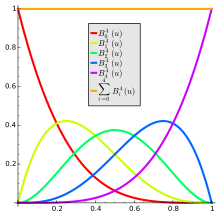
\includegraphics[height=1.5in]{figures/background/Bernstein_curves.png}
    \end{subfigure}%
    ~ 
    \begin{subfigure}[t]{0.5\textwidth}
        \centering
        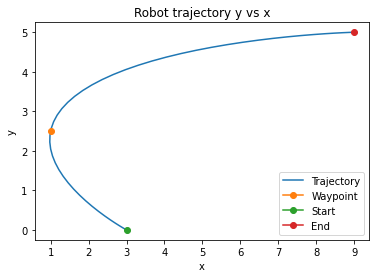
\includegraphics[height=1.5in]{figures/background/holonomic_Bernstein.png}
    \end{subfigure}
    \caption[Bernstein curves and trajectory]{(a) Bernstein basis curves of order-4, (b) An example of a holonomic robot trajectory fitted using order-4 Bernstein polynomials.}
    \label{fig:Bernstein_curv}
\end{figure*}

The trajectory represented as a Bernstein polynomial can be depicted in terms of the basis polynomials and Bernstein coefficients $W_i$ as follows:

\begin{equation}
    f(t) = \sum_{i=0}^{n}W_i \boldsymbol{B_{i,n}(t)}
    \label{eqn:Bernstein}
\end{equation}

The derivatives of the Bernstein basis function are, in themselves, Bernstein polynomials\cite{bernstein_gen}. Similar to eqn. \ref{eqn:cubic_spline}, we can equate the function $f$ at discrete timestamps to obtain the Bernstein coefficients $W_i$ by solving a system of linear equations.

\subsection{Discrete-time representation}

A discrete-time trajectory is represented as a sequence of values $f(t) = \{f(t_0), f(t_1), ... f(t_f)\}$ corresponding to successive timestamps $t = \{t_0, t_1, ... t_f\}$. It can be thought of as sampling a continuous-time trajectory function at predefined timestamps. For the purpose of computational representation of trajectories, discrete-time sequences are generally used. To represent a trajectory in continuous time, generally, the basis functions are predetermined and only the coefficients are saved to reconstruct the trajectory as a weighted linear combination of known basis functions, similar to eqns. \ref{eqn:cubic_spline} and \ref{eqn:Bernstein}.


\section{Posing trajectory planning as an Optimization Problem}
\label{sec:optimization-intro}
\textbf{Linear Programming:}
Solving polynomial coefficients for the boundary state constraints as discussed in section \ref{sec:trajectory_rep} falls into a class of mathematical optimization known as Linear Programming(LP), which, simply put, involves solving a system of linear equations. Eqn. \ref{eqn:LP} with the polynomial weight vector as $W$, the basis polynomial matrix as $B$ and the right-hand side boundary vector $A$ can be solved using LP as follows:
\begin{equation}
    W = inv({B})A
\end{equation}

In addition to solving for boundary constraints, we can define a general objective function($\zeta$) in terms of the trajectory function $f$ that should be subject to the robot's kinematic, dynamic, and environmental equality and inequality constraints $g$. Mathematically, this optimization problem may be written as:

\begin{equation}
\min_{f(t)} \zeta(f(t)) \qquad \text{st: } g(f(t)) \leq 0
\end{equation}


\textbf{Quadratic Programming:}
For most path planning objectives such as goal-reaching, jerk minimization, and smooth trajectory generation, the cost function $\zeta$ is quadratic with respect to $f$, giving rise to constrained Quadratic Program(QP) optimization, and can be written as follows:


\begin{equation}
\min_{f} \frac{1}{2}f^{T}\boldsymbol{P}f + q^{T}f \qquad
 \text{st: }  Gf \leq h\label{eqn:QP}
\end{equation}

For example, the objective function could be the Euclidean distance of the current position of a robot from the intended goal position, and the constraint matrices $G$ and $h$ could denote the boundary states and velocity limits for the robot. The solution to the above QP optimization problem presents challenges, including the non-convexity of the objective function and its constraints and discontinuities in the objective function. We will now discuss two approaches to solving QP optimization.

\subsection{Gradient-based Optimization}\label{sec:gradient-optim}
The QP optimization proposed in eqn. \ref{eqn:QP} for $\zeta(f) = \frac{1}{2}f^TPf + q^Tf$ can be solved by finding the inflection point in the convex objective curve. To do this, we compute the gradient of the objective function with respect to the optimization variables as follows:


\begin{equation}
    \triangledown_{f}{\zeta} = f^TP + q^T = 0
    \label{eqn:gradient}
\end{equation}

Now, we attempt to attain the minima by updating the optimization variable with an iterative Gradient Descent approach. The update rule for $f$ in the $k^{th}$ optimization iteration for a learning rate of $\alpha > 0$ is as shown below:

\begin{equation}
    f_{k+1}^T = f_k^T - \alpha \triangledown_{f}{\zeta}
\end{equation}

The feasibility of solving the optimization problem with this approach is dependent on factors such as the convexity of the objective function, the convexity of the constraints, and the computational complexity of computing the gradient. A few existing approaches for mobile robot path planning that use gradient-based optimization include \cite{aks_ral21}, \cite{CDC_time_scaling}. Even for manipulator planning, \cite{CHOMP}, \cite{STOMP} use gradient-based optimization where the gradient of the objective is computed over the joint angle space. 

\subsection{Sampling-based Optimization}\label{sec:sampling-optim}

Sampling-based approaches bypass the gradient computation in eqn.\ref{eqn:gradient} by sampling random points in the solution space and picking the sample that minimizes the optimization objective $\zeta$. This approach is adopted in Rapidly-Exploring Random Trees(RRT) \cite{RRT-og}, where around each current point, random uniform samples of points are considered and connected to an expanding tree towards the goal. Similarly, in A* \cite{A*}, Djikstra, and EBS-A* \cite{EBS-A*} algorithms, a heuristic function is optimized over an expanding graph search to compute the most optimal path from a start pose to an end pose. 

Recent approaches \cite{STORM}, \cite{iCEM} and \cite{VPSTO} sample candidate solutions to the optimization problem from a distribution and compute the cost associated with each candidate. Then the sample distribution is adapted to produce a "better" sample in the next iterations. This translates a deterministic optimization problem into a stochastic optimization problem. The benefit of this approach is its speed and generalizability to non-convex, discontinuous objective functions that would be infeasible to solve using gradient-based optimization techniques. 

\subsection{Collision Avoidance methods}

Collision avoidance for a robot involves the interaction of the robot with its environment and ensuring the following:

\begin{enumerate}
    \item Collision avoidance with static obstacles (e.g, tree on a road, brick wall, etc.)
    \item Collision avoidance with dynamic obstacles (e.g, other moving robots, pedestrians (for cars), birds (for drones) etc.)
    \item \label{point:self-collision}Self-collision avoidance in case of an extended robot, such as a manipulator, between its own links and joints.
\end{enumerate}

Collision detection is usually performed by sensors onboard the robot in simulation or hardware, but for the purpose of path planning, we mathematically estimate collisions using geometric approximations of obstacles and the robot. We assume the map of the environment is known to the robot from the Localization and Mapping modules. Most existing research, such as \cite{RVO}, approximate obstacles of varied shapes by their circumscribing spheres in 3-D or circles in 2-D. The robot itself is reduced to a point object, while its circumscribing radius is added as padding to the obstacles in the environment to account for grazing scenarios to simplify the path-planning process and collision detection. \cite{aks_ral21} estimates obstacles with axis-aligned ellipsoids with padding to generalize to a wider range of obstacles with non-uniform dimensions. 

\subsubsection{Distance-based Collision Avoidance}\label{sec:distance-based-collision}

\textbf{For Mobile Robots:}
For a 2-D mobile robot centered at $(x_r, y_r)$, let us consider a circumscribing circle of radius $R_{bot}$. We aim to avoid collision with an obstacle centered at $(x_o, y_o)$ of a circumscribing radius of $R_{obs}$. To avoid collision of the robot with the obstacle, we need to ensure the Euclidean distance between their centers is greater than or equal to the sum of their radii (the equality holding in the situation where the robot just grazes along the obstacle). Mathematically this can be represented as follows:

\begin{equation}
    \sqrt{(x_r - x_o)^2 + (y_r - y_o)^2} \geq R_{obs}+R_{bot}
\end{equation}

For unequal robot dimensions along the axes, we can estimate the robots with their circumscribing ellipsoids instead of spheres in 3-D. Fig \ref{fig:robot-ellipsoidals} depicts the axis-aligned ellipsoidal robot representation and the distance between them that we use in Chapter \ref{ch:gpu_mat} for our multi-agent optimizer.

\begin{figure}[ht]
    \centering
    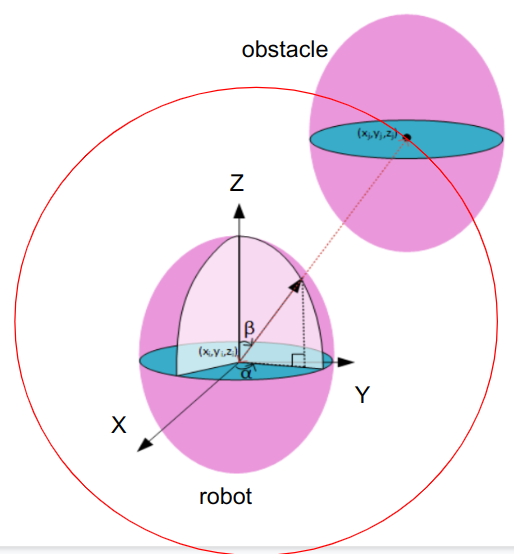
\includegraphics[scale=0.5]{figures/background/ellipsoidals.png}
    \caption[Ellipsoidal Robots]{Axis-aligned ellipses representing robots for collision avoidance in chapter \ref{ch:gpu_mat}.}
    \label{fig:robot-ellipsoidals}
\end{figure}

\textbf{For Manipulators:}
The same approach can be extended to robots moving in higher dimensional spaces. For complex robot systems such as manipulators, distance-based collision avoidance involves self-collision among the robot links, as discussed in point \ref{point:self-collision}, along with collision avoidance with the environment. Based on our literature survey, there are broadly three approaches to solving this problem:
\begin{enumerate}
    \item \label{point: SDF} \textit{Distance of sampled points:} \cite{STOMP} approximates the robot body $B$ as a set of overlapping spheres $b \in B$ of radius $r_l$. We require all points in each sphere to be a distance, at least $\epsilon$ away from the closest obstacle. This constraint can be simplified as the center of the sphere being at least $\epsilon + r_l$ away from obstacles. Thus, our obstacle cost function is as follows:
    \begin{equation}
        q_o(\theta_t) = \sum_{b \in B}{max(\epsilon+r_l - d(x_b),0)||\dot{x_b}||}
    \end{equation}
    
    \item \textit{Implicit Representation Learning-based Collision Avoidance:} \cite{STORM} uses \textit{jointNERF}, a query-able neural network that learns implicit representations of the objects in the environment, including robot links and obstacles, and computes distances between them to detect collisions. 
    
 
\end{enumerate}

This dissertation addresses collisions for manipulators by involving mesh overlaps for collision avoidance in manipulators using the PyBullet simulator. 

\subsubsection{Time-scaling}

A change in the independent variable from $t$ to $\tau$ in the trajectory definition $f(t)$ does not change the path taken by the robot, but brings the following changes in the velocity profile of the trajectory:

\begin{equation}
    \dot{f(\tau)} = \dot{f(t)}\frac{dt}{d\tau}
\end{equation}

The trajectory $f(\tau)$ can be thought of as the robot passing through the same points as $f(t)$, with a scaled version of the original velocity $\dot{f(t)}$, i.e. changing the velocity and acceleration of the robot while keeping its position undisturbed. This transformation in the time scale allows us to regulate the velocity of the robot, playing a key role in collision avoidance. The robot sticks to its original planned global path with a scaled version of its original velocity, and regains its original velocity once the collision with a dynamic obstacle has been avoided. This approach proves to be agnostic to the kinematics of the robot itself since it does not hold any assumptions about the initial trajectory of the robot.

As for the transformation between $t$ and $\tau$, \cite{CDC_time_scaling} experiments with constant as well as exponential time-scaling, estimating the parameters of the transformation function and using them for collision avoidance against workspaces cluttered with dynamic obstacles.

\subsection{Performance Metrics}\label{sec:traj_eval_metrics}

This subsection discusses a few performance metrics that are used to evaluate trajectories obtained from different planning methods. We use the following metrics for bench-marking one algorithm against another:

\begin{itemize}
\item \textit{Smoothness cost:} It is computed as the norm of the second-order finite-difference of the robot position at different time instances. We aim to minimize this smoothness cost to get smooth trajectories feasible for execution through a controller. 
\item \textit{Arc-length:} It is computed as the norm of the first-order finite-difference of the robot positions at different time instances. We aim to minimize arc-length for computed trajectories to ensure short trajectory curves are returned.
\item \textit{Computation Time:} The time taken for each approach to return a smooth and collision-free solution. Depending on the application, we may want computation time in the order of milliseconds for real-time online adaptive planning or in the order of a few seconds for offline planning. 
\item \textit{Success Rate:} It is computed as the number of successful completion of the intended task (such as, reaching a goal, picking up a payload) as a fraction of the total number of tries. An algorithm with a higher success rate will be preferred for the task at hand.
\item \textit{Number of Collisions:} It is calculated as the number of times the robot collides with static and dynamic obstacles, as well as with itself while following a planned trajectory. Lower the number of collisions, the more effective our planning method.
\end{itemize}

\section{Multi-Robot Path Planning}

This section provides a brief overview of the multi-robot path planning problem, including a primer for some of the ideas that shape our algorithm discussed in Chapter \ref{ch:gpu_mat}. 

\subsection{Applications}

Multi-robot systems consist of several interaction-aware robots, each capable of independent decision-making to execute a collective task. The inspiration behind such systems is derived from swarms of bees and other insects. Typical examples of such systems used widely include swarm drones and robot fleets. Multi-robot systems involve coordination and communication among constituent robots, allowing a division of labor to achieve a given task. For example, robot fleets are being extensively used today to perform search-and-rescue missions in areas unsuitable for human intervention, particularly during natural disasters. Swarm drones are also used for imaging and mapping vast territories, particularly for military applications to detect enemy advances. They are also used for demonstrating geometric formations, as well as for military combat, last-mile parcel delivery, and precision agriculture. 

\begin{figure}[ht]
    \centering
    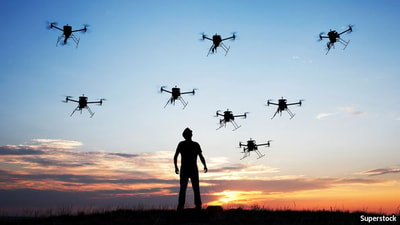
\includegraphics[scale=0.5]{figures/background/swarm_drones.jpg}
    \caption[Swarm Drones]{Swarm drones are used for a wide variety of robotics applications, ranging from search-and-rescue missions, military combat, parcel delivery, and precision agriculture. Source: \scriptsize{\url{https://www.economist.com/the-economist-explains/2015/10/02/how-swarm-drones-are-mimicking-nature}}}
    \label{fig:swarm-drones}
\end{figure}

\subsection{Challenges Involved}

A multi-robot system must ensure that individual robots do not crash into their surroundings or each other. The whole system must also act and make decisions rapidly within the limits of the processors and information available to each drone. A few challenges associated with multi-robot control and coordination:

\begin{enumerate}
    \item \textit{Communication and bandwidth limitations:} Individual robots need to communicate with each other and with a central ground station to share information and coordinate their actions. However, communication and bandwidth limitations can cause delays and disruptions in data transmission. 

    \item \textit{Decentralized control:} Multi-robot systems typically use decentralized control, meaning that each drone makes decisions based on local information and without central coordination. This gives rise to the need for predictive modeling of other agents' behaviors, which can lead to conflicts and coordination problems.

    \item \textit{Sensing and perception:} Multi-robot systems need to perceive their environment accurately to avoid collisions and perform their tasks effectively. However, the limited sensing capabilities of robots and the complexity of the environment can make it difficult to obtain reliable information about the surroundings. Moreover, as the number of drones in a swarm increases, the overhead for collision avoidance also increases since collision constraints need to be computed pairwise.

    \item \textit{Task allocation and optimization:} The optimal allocation of tasks among multi-robot systems can be challenging, particularly when the tasks have different priorities or require different resources. Moreover, the dynamic nature of many applications means that the tasks and their priorities may change over time, requiring continuous adaptation and re-planning.
    
\end{enumerate}

Overall, multi-robot planning and coordination are complex and challenging tasks that require careful consideration of communication, sensing, control, and optimization. Despite these challenges, the potential benefits of swarm drones make them an attractive area of research and development for many applications.

\subsection{Graph-Search-based Multi-Agent Path Finding}\label{sec:MAPF}

Multi-Agent Path Finding(MAPF) consists of a class of algorithms under the umbrella of multi-robot planning that involves the computation of collision-free paths from the start to the goal in a shared environment. Typical solutions for the multi-agent path-finding problem derive inspiration from shortest path computation in graph theory by discretizing the action space of the robots into graph nodes and constructing edges between them based on permissible controls. Let us now discuss some of the different graph-search-based algorithms that have been developed for MAPF:

\subsubsection{A* Algorithm:}\label{sec:A*}
A*\cite{A*} is a popular heuristic search algorithm that can be used for MAPF. It uses an admissible heuristic function to estimate the cost of reaching the goal state, typically based on the distance between agents and their targets. A* algorithm can find optimal solutions but can be slow for large-scale MAPF problems.

\subsubsection{Conflict-based Search(CBS) Algorithm:}
CBS\cite{CBS} is a popular algorithm for solving MAPF problems. CBS is a two-level search algorithm that first searches for individual agent paths and then resolves conflicts between them. CBS can handle a large number of agents and can find optimal solutions for MAPF problems.


\subsubsection{Push and Swap (PaS):}
PaS\cite{PaS} is a local search algorithm that operates by pushing agents and swapping their positions to find a collision-free solution. PaS algorithm is efficient for small-scale MAPF problems but can struggle to find optimal solutions for large-scale problems.

\subsection{Batch Trajectory Optimization}

Batch trajectory optimization can be applied to multi-robot systems, where a group of robots works together to perform a task. In this context, the goal is to optimize the trajectories of all robots in the system to achieve the desired task while minimizing the overall cost of the system. Instead of considering all the robots in the system at once, they could be split into groups or batches that solve the trajectory optimization problem independent of one another as well. A set of candidate trajectories are chosen for each robot based on the robot dynamics and task definition and are optimized for all the robots in a single shot by minimizing the overall cost function for all the robots in the system. The cost function could the the norm of the acceleration of all the robots to ensure precise, smooth movements, or the total time taken by all the robots to execute the given task. Note that this optimization problem also includes collision avoidance constraints between pairs of agents and obstacles in the environment. Then the optimal set of trajectories are executed by all the robots. 

\subsection{Matrix operations on a GPU}

Matrix computations can be sped up over a GPU (Graphics Processing Unit) by taking advantage of the massively parallel architecture of the GPU. A GPU typically contains thousands of small processing cores that work together to perform computations in parallel. Matrix computations, such as matrix multiplication, are particularly well-suited for parallel processing because each element of the output matrix can be computed independently.

To speed up matrix computations on a GPU, the matrix data is first transferred from the CPU memory to the GPU memory. This transfer can be done using specialized libraries such as CUDA, which is a parallel computing platform and programming model developed by NVIDIA for general-purpose computing on GPUs. Once the matrix data is in the GPU memory, the computation is split into many smaller computations that can be performed in parallel across the thousands of cores on the GPU. For example, in matrix multiplication, each output element can be computed by multiplying the corresponding row of the first matrix by the corresponding column of the second matrix. By breaking the computation down into smaller tasks that can be performed in parallel, the GPU can perform matrix computations much faster than a CPU, which typically has fewer processing cores.

We use the JAX library \cite{bradbury2020jax}, developed by Google in Chapter \ref{ch:gpu_mat} to accelerate matrix operations. Additional details and usage of the JAX NumPy library has been discussed in Appendix \ref{appendix:JAX}



\section{Manipulator Path Planning}

This section provides a brief overview of the kinematics of robot manipulators and introduces the task of path planning for manipulators, as a background for our approach discussed in Chapter \ref{ch:bl_arm}.

The problem of robot manipulator path planning is the task of finding a collision-free path for a robotic arm to move from its initial position to a desired final position while avoiding obstacles in its workspace. This is a challenging problem because the workspace of the robot can be complex and high-dimensional, and the motion of the robot can be constrained by its physical limits, such as joint velocity and angle limits. Path planning algorithms must take into account these constraints and find an optimal path that satisfies the constraints while minimizing some performance criteria, such as the path length or the time required to complete the motion. This problem is relevant in many applications of robotics, including industrial automation, manufacturing, and healthcare, where robots are used to perform repetitive or complex tasks in a safe and efficient manner. An example of path planning required for a robot manipulator is illustrated in Figure \ref{fig:manipulator-planning}.

\begin{figure}[ht]
    \centering
    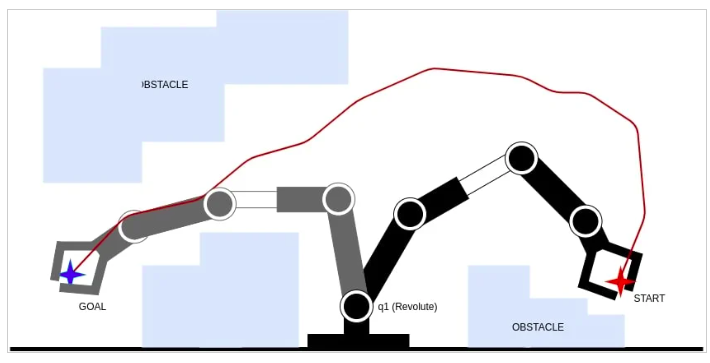
\includegraphics[scale=0.5]{figures/background/manipulator_planning.png}
    \caption[Path Planning for a Manipulator]{An illustration showing the task of path planning for a robot manipulator from a start pose to an end pose, while avoiding obstacles in the surroundings and preventing self-collisions and coiling in on itself. The red line denotes the trajectory to be followed by the end-effector from start to goal. Source: \scriptsize{\url{https://control.com/technical-articles/how-does-motion-planning-for-autonomous-robot-manipulation-work/}}}
    \label{fig:manipulator-planning}
\end{figure}

\subsection{Manipulator Kinematics}\label{sec:bg-manipulator-kinematics}

In the context of this thesis, we discuss the manipulator planning problem primarily for two robot manipulators - Franka Emika Panda robot arm and Universal Robots(UR5e) robot arm. The number of degrees of freedom(DoF) for the former is 7, while that for the latter is 6. Figure \ref{fig:Franka-Panda} shows the Franka Panda robot manipulator against its links and joints, while Figure \ref{fig:ur5e} denotes the same for the UR5e robot arm. 

\begin{figure*}[t!]
    \centering
    \begin{subfigure}[t]{0.4\textwidth}
        \centering
        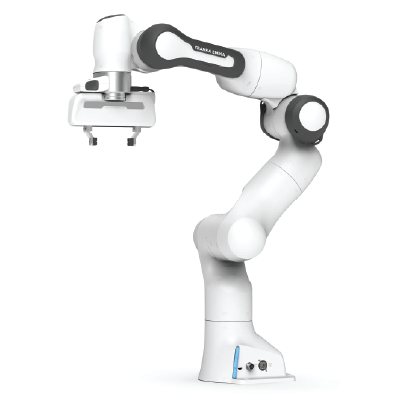
\includegraphics[height=1.5in]{figures/background/franka_overview.png}
    \end{subfigure}%
    ~ 
    \begin{subfigure}[t]{0.5\textwidth}
        \centering
        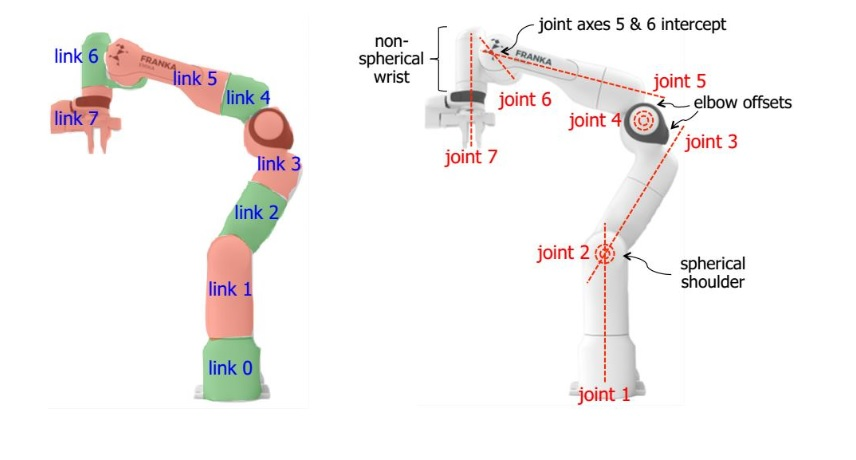
\includegraphics[height=1.5in]{figures/background/franka_links.png}
    \end{subfigure}
    \caption[Franka Emika Panda Robot Arm]{(a) The Franka Emika Panda Robot Arm with an end-effector(two-finger gripper)(b) The links and types of joints and their locations for the 7-DoF Franka Panda manipulator.}
    \label{fig:Franka-Panda}
\end{figure*}

The kinematics of a robot manipulator describes the relationship between the joint angles and the position and orientation of the end-effector of the robot. Forward kinematics denotes the transformation of joint angles to an end-effector position, while inverse kinematics attempts to calculate the required joint angles to achieve a desired end-effector position. We will now discuss the forward kinematics of both manipulators mathematically.

\subsubsection{Franka Emika Panda}

The Franka Emika Panda is a 7 degree-of-freedom robot manipulator that is widely used in research and industrial applications. The Panda robot has a serial kinematic structure, where each joint is connected to the previous joint and to the base of the robot. The joint angles, corresponding to the 7 joints, shown in Figure \ref{fig:Franka-Panda} are denoted by $q_1$, $q_2$, ..., $q_7$, corresponding to the rotations of each joint around its respective axis. The position and orientation of the end-effector are represented by a $4$x$4$ transformation matrix $T$. The forward kinematics of the Panda robot can be described by the following equations:

\begin{equation}
    T = T_1T_2T_3T_4T_5T_6T_7
    \label{eqn: fk_manipulator}
\end{equation}


where $T_i$ is the transformation matrix corresponding to the $i^{th}$ joint of the robot. These transformation matrices can be computed from the Denavit-Hartenberg parameters, which describe the geometry and kinematics of the robot. The Denavit-Hartenberg frames and parameters for the Franka Panda robot arm are depicted in Figure \ref{fig:dh-franka}.

\begin{figure}[ht]
    \centering
    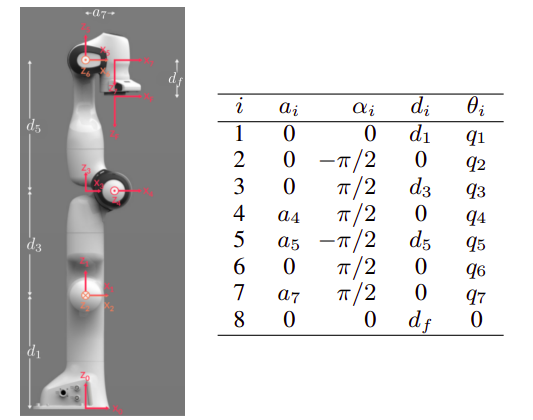
\includegraphics[scale=0.5]{figures/background/dh-franka.png}
    \caption[DH Parameters for the Franka Panda Arm]{Denavit-Hartenberg(D-H) frames and parameters for the 7-DoF Franka Panda robot arm. Source: \cite{DH-Franka}.}
    \label{fig:dh-franka}
\end{figure}

\subsubsection{UR5e}

\begin{figure*}[t!]
    \centering
    \begin{subfigure}[t]{0.4\textwidth}
        \centering
        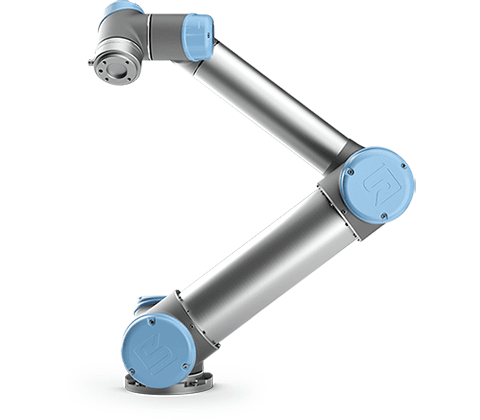
\includegraphics[height=1.5in]{figures/background/ur5e_overview.png}
    \end{subfigure}%
    ~ 
    \begin{subfigure}[t]{0.5\textwidth}
        \centering
        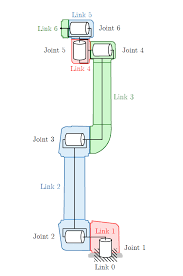
\includegraphics[height=1.5in]{figures/background/ur5e_links.png}
    \end{subfigure}
    \caption[Universal Robots(UR5e) Robot Arm]{(a) The Universal Robots(UR5e) Robot Arm (b) The links and types of joints and their locations for the 6-DoF UR5e manipulator.}
    \label{fig:ur5e}
\end{figure*}

The Universal Robots UR5e is a 6-degree-of-freedom robot arm. The joint angles, corresponding to the 6 joints, shown in Figure \ref{fig:ur5e} are denoted by $q_1$, $q_2$, ..., $q_6$, and the overall forward kinematics is described by the serial multiplication of six transformation matrices corresponding to the six joints, similar to eqn.\ref{eqn: fk_manipulator}. The Denavit-Hartenberg(D-H) frames and parameters for the 6-DoF UR5e robot arm are depicted in Figure \ref{fig:dh-ur5}.

\begin{figure*}[t!]
    \centering
    \begin{subfigure}[t]{0.5\textwidth}
        \centering
        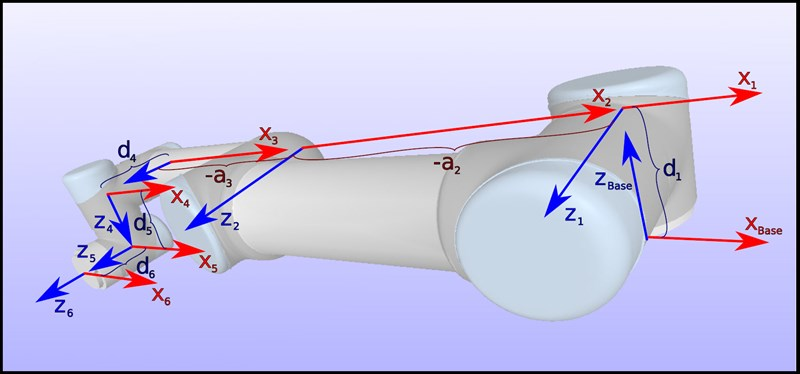
\includegraphics[height=1.5in]{figures/background/dh_ur5ea.jpg}
    \end{subfigure}%
    ~ 
    \begin{subfigure}[t]{0.3\textwidth}
        \centering
        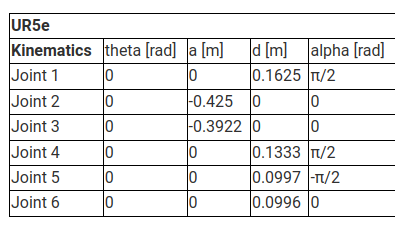
\includegraphics[height=1.5in]{figures/background/dh_ur5eb.png}
    \end{subfigure}
    \caption[DH Parameters for the UR5e Arm]{Denavit-Hartenberg(D-H) frames and parameters for the 6-DoF UR5e robot arm. Source: \scriptsize{\url{https://www.universal-robots.com/articles/ur/application-installation/dh-parameters-for-calculations-of-kinematics-and-dynamics}}}
    \label{fig:dh-ur5}
\end{figure*}

\subsection{Challenges Involved}

Path planning for robot manipulators is a complex problem that involves several challenges. Here are some of the key challenges involved:

\begin{itemize}
    \item \textit{High Dimensionality:} Robot manipulators typically operate in high-dimensional spaces, with each joint providing a degree of freedom, such as the 7-dimensional joint angle space in the case of the Franka Panda arm and the 6-dimensional joint space for the UR5e arm. This makes the search space for path-planning algorithms very large, and finding an optimal path becomes computationally expensive.
    \item \textit{Nonlinear Constraints:}  The motion of robot manipulators is subject to nonlinear constraints, such as the dynamics of the robot and the workspace bounds, as well as physical constraints, such as joint limits and collision avoidance. Incorporating these constraints into path-planning algorithms can be challenging, and some algorithms may require sophisticated mathematical techniques to solve the constraints.
    \item \textit{Real-time Operation:}  In many rearrangement applications, path planning must be performed in real-time, with the manipulator making decisions and adapting to new obstacles or changes in the environment. Real-time path planning requires efficient algorithms that can quickly search the space of possible paths and adapt the plan as needed.
\end{itemize}

Overcoming the above challenges requires the development of efficient path-planning algorithms that can handle these constraints and produce high-quality paths. We attempt to address all these challenges through our bi-level trajectory optimizer for manipulators discussed in Chapter \ref{ch:bl_arm}.

\subsection{Joint space-vs end-effector space}

For a robot manipulator, the path-planning can be performed in two motion spaces - either in the high-dimensional space formed by the joint angles corresponding to each movable joint or the end-effector space, which is a 3-dimensional space limited by the workspace bounds  or a 2-dimensional table plane (for planar end-effector motion). The choice of motion space is determined by the requirements of the task at hand. For example, for a robot arm pushing objects on the table, the major task at hand involves the pose of the end-effector on the 2-D tabletop plane, and hence the path planning can be performed in the Cartesian end-effector space or even in the Cartesian space of the center of the object being pushed on the table. For tasks involving grasping objects, it is more effective to plan trajectories in the joint space in order to avoid collisions and minimize joint movements. 

Based on the two paradigms of optimization discussed in Sections \ref{sec:gradient-optim} and \ref{sec:sampling-optim}, let us discuss both Gradient-based and Sampling-based trajectory optimization for a robot manipulator.

\subsection{Gradient-based Optimization}\label{sec:bg-gradient-manipulator}

\subsubsection{CHOMP}\label{sec:CHOMP}

CHOMP (Covariant Hamiltonian Optimization for Motion Planning)\cite{CHOMP} is a gradient-based optimization method for efficient motion planning of robot manipulators in high-dimensional spaces. This method was developed by Brian Paden and Emo Todorov in 2011.

The key idea behind CHOMP is to formulate the motion planning problem as an optimization problem, where the objective is to minimize an objective function that typically includes terms that penalize collisions with obstacles, deviation from a desired trajectory, and energy consumption. In CHOMP, the optimization is performed using a gradient descent method, where the gradient of the cost function with respect to the joint angles of the robot is computed and used to update the joint angles iteratively. The gradient is computed using backpropagation through time, which involves propagating the gradient backward through a sequence of time steps.

One of the key advantages of CHOMP is its ability to handle non-convex constraints and to generate smooth, continuous paths that avoid collisions with obstacles. This is achieved by using a smoothing term in the cost function, which encourages the joint angles to vary smoothly over time. Another advantage of CHOMP is its scalability to high-dimensional spaces, which makes it well-suited for motion planning of robot manipulators with many degrees of freedom.

However, CHOMP does have some limitations. It requires a good initial guess of the path, which can be challenging in complex environments with many obstacles. The optimization can also converge to local minima, which can result in suboptimal paths. Further, CHOMP involves gradient computations which may get intractable to compute in very high-dimensional spaces and spend a significant amount of time to return a feasible trajectory, eliminating the scope of real-time path planning. To address these limitations, various extensions and modifications to CHOMP have been proposed, such as incorporating stochastic optimization or combining CHOMP with other planning algorithms.


\subsubsection{TrajOpt}\label{sec:TrajOpt}

TrajOpt\cite{TrajOpt}, developed by John Schulman and his colleagues at UC Berkeley in 2013, is an open-source library for motion planning and trajectory optimization of robot manipulators.

TrajOpt also involves gradient-based trajectory optimization using techniques such as sequential quadratic programming or gradient descent. The TrajOpt library provides a flexible and modular framework for specifying the motion planning problem, allowing users to define a wide range of cost functions and constraints, including collision avoidance, joint limits, end-effector constraints, and task-specific objectives such as minimizing energy consumption. TrajOpt also uses a collision-checking algorithm based on bounding volume hierarchies, which can quickly identify potential collisions between the robot and the environment. It also incorporates a warm-starting strategy, which initializes the optimization algorithm with a feasible solution from a previous iteration, reducing the time required for convergence.

TrajOpt, written in C++ and Python, is designed to be highly customizable and extensible. It can be integrated with various robot simulation and control frameworks, such as ROS, Gazebo, or PyBullet, and supports a wide range of environments, robot models, and kinematic solvers. \cite{OpenRAVE} uses TrajOpt as a collision-detection module.

\subsection{Sampling-based Optimization}\label{sec:bg-sampling-manipulator}

Sampling-based optimizers rely on stochastic optimization, i.e. sampling a set of potential candidate trajectories to be followed by the manipulator and evaluating the associated costs to finally choose the trajectory with the minimum cost. The best set of candidates is used to iteratively improve on the samples for the next iteration, ultimately helping the optimizer converge to an optimum in the cost function. 

\subsubsection{STORM}

STORM(Stochastic Tensor Optimization for Robot Motion)\cite{STORM} is an optimization algorithm designed to efficiently and effectively generate smooth and collision-free trajectories for robots in complex environments between a start state and a desired state by iteratively optimizing a tensor-based cost function. STORM works by first defining a tensor-based representation of the state space, designed to capture the high-dimensional motion space of the robot. The tensor is defined as a multi-dimensional array, where each dimension corresponds to a specific aspect of the robot's state, such as position, velocity, or acceleration. The size of each dimension is determined by the resolution of the state space.

The optimization process is stochastic, which means that it involves randomly sampling different trajectories and evaluating their costs. Self-collisions are detected by using \textit{jointNERF}, a network that computes the closest distance between robot links given joint poses, while environment collisions are based on signed distances. This randomness helps to ensure that STORM is able to find a diverse set of trajectories that can be used to navigate complex environments. Additionally, STORM is able to leverage parallel computing to speed up the optimization process, which can be critical for real-time applications.

One of the key advantages of STORM is its ability to handle high-dimensional state spaces, which is particularly useful for manipulator path planning. It achieves this by using a tensor-based representation of the state space, which allows it to efficiently explore large and complex environments. STORM is also able to incorporate a wide range of constraints, including collision avoidance, joint limits, and kinematic constraints.

\subsubsection{Cross-Entropy Methods(CEM)}

The cross-entropy method (CEM)\cite{CEM_og} is a derivative-free optimization technique that employs an adaptive importance sampling procedure using the cross-entropy measure. In each iteration of the CEM-based stochastic trajectory optimization, the following two steps are performed:

\begin{itemize}
    \item Derive candidate trajectories by sampling from a probability distribution
    \item Minimize the cross-entropy between the sample distribution and a target distribution to update the parameters of the former.
\end{itemize}

Mathematically, these steps can be represented as follows (Source: \url{https://en.wikipedia.org/wiki/Cross-entropy_method}):

\begin{enumerate}
    \item Choose initial parameter vector $\boldsymbol{v}^{0}$; set t = 1
    \item \label{point:sampling}Generate a random sample $\boldsymbol{X_1}$, ...,$\boldsymbol{X_N}$ from $f(\boldsymbol{v^{(t-1)}})$.
    \item Solve for $\boldsymbol{v^{(t)}}$, for a given cost function $\zeta$ where,
    \begin{equation}
        \boldsymbol{v^{(t)}} = \argmax_v\frac{1}{N}\sum_{i=1}^{N}\zeta(\boldsymbol{X_i})\frac{f(\boldsymbol{X_i};u)}{f(\boldsymbol{X_i},\boldsymbol{v^{(t-1)}})}\text{log}f(\boldsymbol{X_i};\boldsymbol{v})
    \end{equation}
    \item If convergence is reached, then stop, otherwise proceed to the next iteration by incrementing $t$ by 1 and repeat from step \ref{point:sampling}.
\end{enumerate}

The cost function $\zeta$ takes into account factors such as the length of the path, the amount of time it takes to complete the path, and the distance from the robot arm to obstacles in the environment. Over time, the CEM algorithm converges to an optimal solution, which represents the best path for the robot arm to reach the target point while avoiding obstacles. 

We use an improved version of CEM, called Via-Point Stochastic Trajectory Optimization(VP-STO)\cite{VPSTO} for manipulator path planning in Chapter \ref{ch:bl_arm}.